% Standalone TikZ sequence diagram: Service-to-DB integration (Agent 1).
% Compile with: pdflatex Seq_Agent1_ServiceToDB.tex
% Export to PNG if needed for inclusion in other tools.
\documentclass[tikz,border=2mm]{standalone}
\usepackage{tikz}
\usetikzlibrary{arrows.meta}
\begin{document}
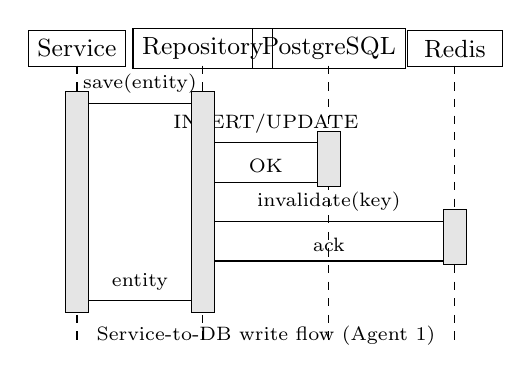
\begin{tikzpicture}[
    every node/.style={font=\small},
    participant/.style={rectangle, draw, minimum width=1.2cm, minimum height=0.45cm},
    arrow/.style={->, >=stealth}
]
    \node[participant] (service) at (0,0) {Service};
    \node[participant] (repo) at (1.6,0) {Repository};
    \node[participant] (db) at (3.2,0) {PostgreSQL};
    \node[participant] (cache) at (4.8,0) {Redis};

    \draw[dashed] (0, -0.22) -- (0, -3.8);
    \draw[dashed] (1.6, -0.22) -- (1.6, -3.8);
    \draw[dashed] (3.2, -0.22) -- (3.2, -3.8);
    \draw[dashed] (4.8, -0.22) -- (4.8, -3.8);

    \draw[arrow] (0, -0.7) -- (1.6, -0.7) node[midway, above, font=\scriptsize] {save(entity)};
    \draw[arrow] (1.6, -1.2) -- (3.2, -1.2) node[midway, above, font=\scriptsize] {INSERT/UPDATE};
    \draw[arrow] (3.2, -1.7) -- (1.6, -1.7) node[midway, above, font=\scriptsize] {OK};
    \draw[arrow] (1.6, -2.2) -- (4.8, -2.2) node[midway, above, font=\scriptsize] {invalidate(key)};
    \draw[arrow] (4.8, -2.7) -- (1.6, -2.7) node[midway, above, font=\scriptsize] {ack};
    \draw[arrow] (1.6, -3.2) -- (0, -3.2) node[midway, above, font=\scriptsize] {entity};

    \draw[fill=black!10] (-0.15, -0.55) rectangle (0.15, -3.35);
    \draw[fill=black!10] (1.45, -0.55) rectangle (1.75, -3.35);
    \draw[fill=black!10] (3.05, -1.05) rectangle (3.35, -1.75);
    \draw[fill=black!10] (4.65, -2.05) rectangle (4.95, -2.75);

    \node[font=\scriptsize] at (2.4, -3.65) {Service-to-DB write flow (Agent 1)};
\end{tikzpicture}
\end{document}
